\documentclass{article}
\usepackage{graphicx} % برای اضافه کردن عکس
\usepackage{amsmath}
\usepackage{listings} % Load the listings package
\usepackage{xcolor}   % Optional: For custom colors
\usepackage{xepersian} % Persian support
\settextfont{XB Niloofar} % Change to a Persian font installed on your system
\setlatintextfont{Courier New} % برای نمایش کدهای انگلیسی

\lstset{
    language=C++,                      % Set language to C++
    basicstyle=\ttfamily\small,        % Use monospaced font
    keywordstyle=\bfseries\color{blue}, % Keywords in bold blue
    stringstyle=\color{red},           % Strings in red
    commentstyle=\itshape\color{green!60!black}, % Comments in green italics
    numbers=right,                     % Line numbers on the right
    numberstyle=\tiny,                 % Line number font size
    stepnumber=1,                      % Show line numbers every line
    frame=single,                      % Add a frame around code
    tabsize=4,                         % Set tab size
    showstringspaces=false,            % Do not show spaces in strings
    xleftmargin=10pt,                  % Adjust left margin for better alignment
    xrightmargin=10pt                  % Adjust right margin for better alignment
}

\begin{document}

\section*{تقدم عملگر‌ها}

در زبان C++ ترتیب و نحوه ارزیابی عملگر‌ها به دو مفهوم تقدم (Precedence) و وابستگی (Associativity) عملگر‌ها وابسته است. هر دو این مفاهیم مرتبط با زمان کامپایل کد هستند.

تقدم عملگرها مشخص می‌کند که در یک عبارت که شامل چندین عملگر است، کدام عملگر ابتدا اجرا شود و وابستگی عملگرها مشخص می‌کند که اگر چندین عملگر با تقدم یکسان در یک عبارت وجود داشته باشند، کدام یک ابتدا ارزیابی شوند.

\begin{figure}[h!]
    \centering
    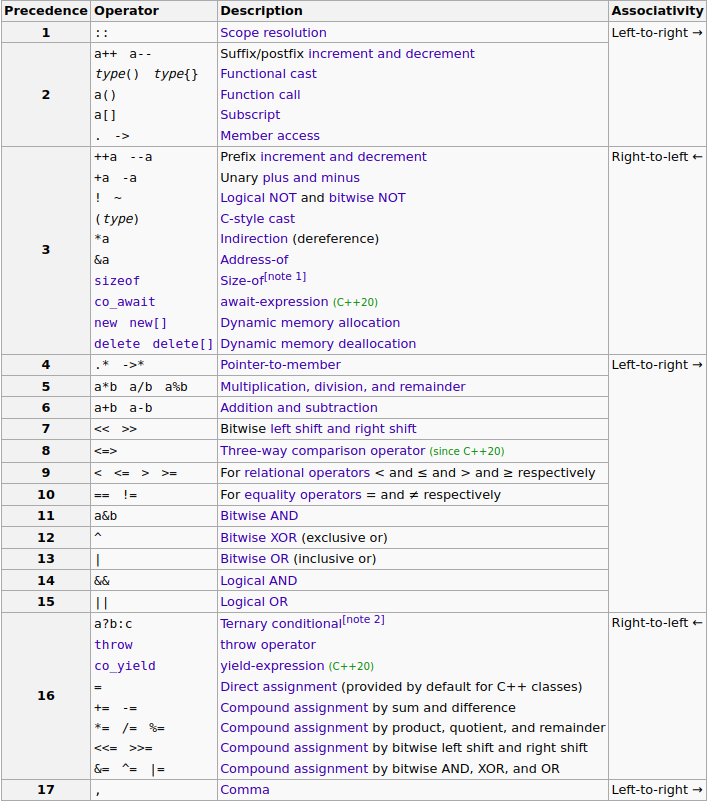
\includegraphics[width=1\textwidth]{Photos/1-operations.png}
    \caption{تمام عملگرهای زبان C++ به همراه تقدم و وابستگی}
    \label{fig:example}
\end{figure}

تقدم عملگر‌ها با بارگذاری بیش از حد عملگر‌ها (operator overloading) تغییری نمی‌کند و ثابت خواهد ماند.
برای نمونه در مثال زیر نحوه ارزیابی مشخص شده است.

\begin{LTR} % Left-to-right environment for code
\begin{lstlisting}
cout << a ? b : c;
\end{lstlisting}
\end{LTR}

\begin{LTR} % Left-to-right environment for code
\begin{lstlisting}
(cout << a) ? b : c;
\end{lstlisting}
\end{LTR}

\section*{گرامر بدون ابهام رعایت تقدم عملگر‌ها}

\begin{table}[h!]
    \centering
    \begin{tabular}{|c|c|}
        \hline
        \textbf{عملگرها} & \textbf{تقدم} \\
        \hline
        \texttt{\&\&}, \texttt{||} & 5 \\
        \hline
        \texttt{\&}, \texttt{|} & 4 \\
        \hline
        \texttt{+}, \texttt{-} & 3 \\
        \hline
        \texttt{*}, \texttt{/} & 2 \\
        \hline
        \texttt{a++}, \texttt{a--} & 1 \\
        \hline
    \end{tabular}
    \caption{تقدم عملگرها در زبان C++}
    \label{tab:operator_precedence}
\end{table}

\begin{align*}
\langle \text{id} \rangle &\to A \mid B \mid C \mid D \mid \dots \\
\langle \text{assign} \rangle &\to \langle \text{id} \rangle = \langle \text{logical-or} \rangle \\
\langle \text{logical-or} \rangle &\to \langle \text{logical-or} \rangle \, || \, \langle \text{logical-and} \rangle \mid \langle \text{logical-or} \rangle \\
\langle \text{logical-and} \rangle &\to \langle \text{logical-and} \rangle \, && \, \langle \text{bitwise-or} \rangle \mid \langle \text{bitwise-or} \rangle \\
\langle \text{bitwise-or} \rangle &\to \langle \text{bitwise-or} \rangle \, | \, \langle \text{bitwise-and} \rangle \mid \langle \text{bitwise-and} \rangle \\
\langle \text{bitwise-and} \rangle &\to \langle \text{bitwise-and} \rangle \, \& \, \langle \text{additive} \rangle \mid \langle \text{additive} \rangle \\
\langle \text{additive} \rangle &\to \langle \text{additive} \rangle \, (+, -) \, \langle \text{multiplicative} \rangle \mid \langle \text{multiplicative} \rangle \\
\langle \text{multiplicative} \rangle &\to \langle \text{multiplicative} \rangle \, (*, /) \, \langle \text{factor} \rangle \mid \langle \text{factor} \rangle \\
\langle \text{factor} \rangle &\to (\langle \text{logical-or} \rangle) \mid \langle \text{id} \rangle \mid \langle \text{id} \rangle++ \mid \langle \text{id} \rangle--
\end{align*}

\section*{معناشناسی عملیاتی بعضی از ساختارها}

\subsection*{تخصیص مقدار به متغیر}
\begin{LTR} % Left-to-right environment for code
\begin{lstlisting}
x = 5;

MOV R1, #5      ; Load the constant 5 into register R1
MOV [x], R1     ; Store the value of R1 into memory at
				 the address of x
\end{lstlisting}
\end{LTR}

\subsection*{جمع دو مقدار}
\begin{LTR} % Left-to-right environment for code
\begin{lstlisting}
z = x + y;

MOV R1, [x]     ; Load the value of x into register R1
MOV R2, [y]     ; Load the value of y into register R2
ADD R3, R1, R2  ; Add the values in R1 and R2, store 
					the result in R3
MOV [z], R3     ; Store the result in memory location z
\end{lstlisting}
\end{LTR}

\subsection*{شرط ساده (if-else)}
\begin{LTR} % Left-to-right environment for code
\begin{lstlisting}
if (x > 0) {
    y = 1;
} else {
    y = -1;
}

MOV R1, [x]      ; Load x into R1
CMP R1, #0       ; Compare R1 with 0
JLE ELSE_LABEL   ; Jump to ELSE_LABEL if R1 <= 0
MOV [y], #1      ; If x > 0, assign 1 to y
JMP END_LABEL    ; Skip the else branch
ELSE_LABEL:
MOV [y], #-1     ; If x <= 0, assign -1 to y
END_LABEL:
\end{lstlisting}
\end{LTR}


\subsection*{حلقه (while)}
\begin{LTR} % Left-to-right environment for code
\begin{lstlisting}
while (x > 0) {
    x = x - 1;
}


LOOP_LABEL:
MOV R1, [x]      ; Load x into R1
CMP R1, #0       ; Compare R1 with 0
JLE END_LABEL    ; Exit the loop if R1 <= 0
SUB R1, R1, #1   ; Decrement R1 by 1
MOV [x], R1      ; Update x in memory
JMP LOOP_LABEL   ; Repeat the loop
END_LABEL:
\end{lstlisting}
\end{LTR}


\subsection*{حلقه (for)}
\begin{LTR} % Left-to-right environment for code
\begin{lstlisting}
for (int i = 0; i < 5; i++) {
    sum = sum + i;
}


; Initialize the loop counter i = 0
MOV R1, #0        ; Load 0 into R1 (i = 0)
MOV [i], R1       ; Store the value of i in memory

; Initialize sum = 0
MOV R2, #0        ; Load 0 into R2 (sum = 0)
MOV [sum], R2     ; Store the value of sum in memory

FOR_LOOP_START:
; Compare i with the upper limit (5)
MOV R1, [i]       ; Load the current value of i into R1
CMP R1, #5        ; Compare i with 5
JGE FOR_LOOP_END  ; If i >= 5, jump to end of the loop

; Add i to sum
MOV R2, [sum]     ; Load the current value of sum into R2
ADD R2, R2, R1    ; Compute sum + i
MOV [sum], R2     ; Store the updated sum back into memory

; Increment i by 1
MOV R1, [i]       ; Load the current value of i into R1
ADD R1, R1, #1    ; Increment i by 1
MOV [i], R1       ; Store the updated value of i in memory

; Jump back to the start of the loop
JMP FOR_LOOP_START

FOR_LOOP_END:
; End of the loop
\end{lstlisting}
\end{LTR}


\subsection*{تعریف و فراخوانی تابع}
\begin{LTR} % Left-to-right environment for code
\begin{lstlisting}
int add(int a, int b) {
    return a + b;
}

int result = add(3, 4);


; Define the function
ADD_FUNC:
PUSH R1          ; Save registers
PUSH R2
ADD R3, R1, R2   ; Compute a + b, store result in R3
POP R2           ; Restore registers
POP R1
RET              ; Return from the function

; Call the function
MOV R1, #3       ; Pass 3 as the first argument (in R1)
MOV R2, #4       ; Pass 4 as the second argument (in R2)
CALL ADD_FUNC    ; Call the add function
MOV [result], R3 ; Store the result in memory
\end{lstlisting}
\end{LTR}


\subsection*{استراکت}
\begin{LTR} % Left-to-right environment for code
\begin{lstlisting}
struct Point {
    int x;
    int y;
};

int main() {
    Point p;
    p.x = 5;
    p.y = 10;
    return 0;
}


main:
    pushq   %rbp                # Save base pointer
    movq    %rsp, %rbp          # Set stack frame
    subq    $16, %rsp           # Allocate 16 bytes on 
    								the stack for 'p'

    movl    $5, -8(%rbp)        # Set p.x = 5
    movl    $10, -4(%rbp)       # Set p.y = 10

    movl    $0, %eax            # Return 0
    leave                       # Restore base pointer
    ret                         # Return
\end{lstlisting}
\end{LTR}


\section*{انقیاد}

\subsection*{انقیاد نوع}
انقیاد نوع به معنی این است که نوع یک متغیر در چه زمانی و چگونه تعیین می‌‌شود. زبان C++ یک زبان انقیاد نوع ایستا است اما در سناریو‌هایی مانند پلی مورفیسم از انقیاد نوع پویا نیز پشتیبانی می‌کند.

\subsubsection*{انقیاد نوع ایستا در C++}
\begin{itemize}
    \item نوع متغیر در زمان کامپایل مشخص می‌شود.
    \item خطاهای مرتبط با نوع در زمان کامپایل بررسی می‌شود.
    \item به دلیل تعیین خطاها و تشخیص نوع‌ها در زمان کامپایل زمان اجرا پایین است.
\end{itemize}

زبان C++ روش‌های مختلفی برای استفاده از این نوع تعریف کرده است:
\begin{itemize}
    \item تعریف متغیر‌ها در برنامه
    \begin{LTR} % Left-to-right environment for code
	\begin{lstlisting}
    int num = 10;        // `num` is bound to type 
    							`// int` at compile-time.
    double pi = 3.14;    // `pi` is bound to type 
    							`// double` at compile-time.
    char ch = 'A';       // `ch` is bound to type `
    							 // char` at compile-time.
	\end{lstlisting}
	\end{LTR}


    \item تعریف توابع عادی در برنامه
    \begin{LTR} % Left-to-right environment for code
	\begin{lstlisting}
void print(int value) {
    std::cout << "Integer: " << value << std::endl;
}

void print(double value) {
    std::cout << "Double: " << value << std::endl;
}

void print(const char* value) {
    std::cout << "String: " << value << std::endl;
}

int main() {
    print(10);               // Resolves to print(int)
    print(3.14);             // Resolves to print(double)
    print("Hello World");    // Resolves to print(const char*)
    return 0;
}
	\end{lstlisting}
	\end{LTR}

 
    \item بارگذاری عملگرها
    \begin{LTR} % Left-to-right environment for code
	\begin{lstlisting}
class Complex {
public:
    double real, imag;

    Complex(double r, double i) : real(r), imag(i) {}

    Complex operator+(const Complex& c) {
        return Complex(real + c.real, imag + c.imag);
    }
};

int main() {
    Complex c1(1.0, 2.0), c2(3.0, 4.0);
    Complex c3 = c1 + c2;    // Operator `+` resolved at compile-time

    std::cout << "Real: " << c3.real << ", Imaginary: " << c3.imag << std::endl;
    return 0;
}

	\end{lstlisting}
	\end{LTR}


    \item قالب‌های توابع (Function Templates)
    \begin{LTR} % Left-to-right environment for code
	\begin{lstlisting}
template <typename T>
T add(T a, T b) {
    return a + b;
}

int main() {
    std::cout << add(3, 4) << std::endl;         // Instantiates add<int>
    std::cout << add(3.14, 1.86) << std::endl;  // Instantiates add<double>
    return 0;
}
	\end{lstlisting}
	\end{LTR}


    \item توابع خطی (inline)
    \begin{LTR} % Left-to-right environment for code
	\begin{lstlisting}
inline int square(int x) {
    return x * x;
}

int main() {
    std::cout << square(5) << std::endl;   // `square(5)` is replaced with `5 * 5` at compile-time
    return 0;
}
	\end{lstlisting}
	\end{LTR}


    \item عبارات ثابت
    \begin{LTR} % Left-to-right environment for code
	\begin{lstlisting}
constexpr int square(int x) {
    return x * x;
}

int main() {
    constexpr int result = square(5);  // Computed at compile-time
    std::cout << result << std::endl;
    return 0;
}
	\end{lstlisting}
	\end{LTR}



    \item توابع کلاس‌ها
    \begin{LTR} % Left-to-right environment for code
	\begin{lstlisting}
class Base {
public:
    void display() {
        std::cout << "Base class display" << std::endl;
    }
};

class Derived : public Base {
public:
    void display() {
        std::cout << "Derived class display" << std::endl;
    }
};

int main() {
    Base obj;
    obj.display();   // Resolves to Base::display() at compile-time
    return 0;
}
	\end{lstlisting}
	\end{LTR}

    \item عبارت‌های لامبدا
    \begin{LTR} % Left-to-right environment for code
	\begin{lstlisting}
int main() {
    auto add = [](int a, int b) { return a + b; };  // Resolved at compile-time
    std::cout << add(3, 4) << std::endl;
    return 0;
}
	\end{lstlisting}
	\end{LTR}

\end{itemize}


\subsubsection*{انقیاد نوع پویا در C++}
\begin{itemize}
    \item نوع متغیر در زمان اجرا مشخص می‌شود.
    \item خطاهای مرتبط با نوع در زمان اجرا بررسی می‌شود.
    \item به دلیل تعیین خطاها و تشخیص نوع‌ها در زمان اجرا زمان اجرا بالا است.
\end{itemize}

زبان C++ به دلیل زمان اجرای پایین این نوع انقیاد روش‌ محدودی را برای استفاده از این نوع تعریف کرده است و آن هم استفاده از توابع مجازی است.

\begin{LTR} % Left-to-right environment for code
\begin{lstlisting}
class Base {
public:
    virtual void display() {  // Virtual function enables dynamic binding
        std::cout << "Base class display" << std::endl;
    }
};

class Derived : public Base {
public:
    void display() override {  // Overrides the base class method
        std::cout << "Derived class display" << std::endl;
    }
};

int main() {
    Base* basePtr;
    Derived derivedObj;
    basePtr = &derivedObj;

    basePtr->display();  // Resolved at runtime to Derived::display
    return 0;
}
\end{lstlisting}
\end{LTR}


\begin{LTR} % Left-to-right environment for code
\begin{lstlisting}
class Animal {
public:
    virtual void speak() = 0;  // Pure virtual function
};

class Dog : public Animal {
public:
    void speak() override {
        std::cout << "Woof!" << std::endl;
    }
};

class Cat : public Animal {
public:
    void speak() override {
        std::cout << "Meow!" << std::endl;
    }
};

int main() {
    Animal* animal;

    Dog dog;
    Cat cat;

    animal = &dog;
    animal->speak();  // Resolved at runtime to Dog::speak

    animal = &cat;
    animal->speak();  // Resolved at runtime to Cat::speak

    return 0;
}	
\end{lstlisting}
\end{LTR}


\section*{مقایسه انقیاد ایستا و پویا}

\begin{table}[h!]
    \centering
    \begin{tabular}{|p{3cm}|p{5cm}|p{5cm}|}
        \hline
        \textbf{ویژگی} & \textbf{انقیاد ایستا} & \textbf{انقیاد پویا} \\
        \hline
        زمان حل اتصال & زمان کامپایل & زمان اجرا \\
        \hline
        عملکرد & بالا (بدون سربار در زمان اجرا) & کمی کندتر (سربار جدول مجازی و RTTI) \\
        \hline
        تشخیص خطا & در زمان کامپایل (ایمن‌تر) & در زمان اجرا (کمتر ایمن) \\
        \hline
        انعطاف‌پذیری & محدود (نوع‌ها در زمان کامپایل ثابت هستند) & بالا (پشتیبانی از چندریختی در زمان اجرا) \\
        \hline
        قابلیت گسترش & نیاز به بازکامپایل برای تغییرات & راحت برای گسترش (مثلاً اضافه کردن کلاس‌های جدید) \\
        \hline
        سهولت در دیباگ & آسان‌تر (رفتار قابل پیش‌بینی است) & دشوارتر (رفتار وابسته به زمان اجرا است) \\
        \hline
        استفاده از حافظه & کم (نیاز به فراداده اضافی نیست) & بیشتر (نیاز به جدول مجازی و RTTI) \\
        \hline
        موارد استفاده & کدهای کارآمد و قابل پیش‌بینی (مثل الگوریتم‌ها) & طراحی انعطاف‌پذیر و قابل گسترش (مثل فریم‌ورک‌ها) \\
        \hline
    \end{tabular}
    \caption{مقایسه انقیاد ایستا و پویا}
    \label{tab:static_dynamic_binding}
\end{table}

\subsection*{انقیاد مقدار یا حافظه}
انقیاد مقدار به معنی این است که نوع یک متغیر در چه زمانی و چگونه به حافظه مقید می‌‌شود. 
زبان C++ از انواع زیر پشتیبانی می‌کند:


\subsubsection*{انقیاد در زمان کامپایل}
\begin{itemize}
    \item آدرس حافظه در زمان کامپایل تعیین می‌شود.
    \item این نوع انقیاد در زبان C++ مرسوم‌‌تر است و برای متغیر‌های محلی و سراسری و ایستا استفاده می‌شود.

\begin{LTR} % Left-to-right environment for code
\begin{lstlisting}
int x = 10;
static int y = 0;
\end{lstlisting}
\end{LTR}
\end{itemize}


\subsubsection*{انقیاد در زمان اجرا}
\begin{itemize}
    \item آدرس حافظه در زمان اجرا مشخص می‌شود.
    \item برنامه‌نویس مسئول آزاد کردن حافظه است.
    \item این نوع انقیاد معمولاً در تخصیص پویا (Dynamic Allocation) با استفاده از دستوراتی مانند new انجام می‌شود.


\begin{LTR} % Left-to-right environment for code
\begin{lstlisting}
int* ptr = new int(10);
\end{lstlisting}
\end{LTR}
\end{itemize}


\subsubsection*{انقیاد موقت}
\begin{itemize}
    \item حافظه به صورت موقت رزرو می‌شود.
    \item این نوع انقیاد زمانی رخ می‌دهد که یک مقدار موقت (temporary) به یک مرجع متصل شود. این اتصال تا زمانی که مرجع در محدوده است، معتبر باقی می‌ماند.


\begin{LTR} % Left-to-right environment for code
\begin{lstlisting}
const int& ref = 42;
\end{lstlisting}
\end{LTR}
\end{itemize}


\subsubsection*{انقیاد پویا با اشاره‌گرهای هوشمند}
\begin{itemize}
    \item آزادسازی حافظه به صورت خودکار توسط اشاره‌گر هوشمند انجام می‌شود.
    \item در C++ مدرن (11 به بعد)، از اشاره‌گرهای هوشمند برای مدیریت انقیاد حافظه به صورت خودکار استفاده می‌شود.
\end{itemize}

\begin{LTR} % Left-to-right environment for code
\begin{lstlisting}
std::unique_ptr<int> ptr = std::make_unique<int>(10);
\end{lstlisting}
\end{LTR}


\section*{تعریف متغیر}
در زبان C++ تعریف متغیر صریح مرسوم است اما ابزاری برای تعریف متغیر ضمنی نیز وجود دارد.

\subsection*{تعریف متغیر صریح}
نوع متغیر به‌طور واضح و صریح در هنگام تعریف مشخص می‌شود.

\begin{LTR} % Left-to-right environment for code
\begin{lstlisting}
int age = 25;          // 'age' is explicitly defined as an integer.
double pi = 3.14;      // 'pi' is explicitly defined as a double.
string name = "John";  // 'name' is explicitly defined as a string.
\end{lstlisting}
\end{LTR}

\subsection*{تعریف متغیر ضمنی}
نوع متغیر برابر با auto قرار می‌گیرد و نوع به‌طور خودکار توسط کامپایلر با توجه به مقدار زمینه تعیین می‌شود.

\begin{LTR} % Left-to-right environment for code
\begin{lstlisting}
auto age = 25;         // The type of 'age' is inferred as int.
auto pi = 3.14;        // The type of 'pi' is inferred as double.
auto name = "John";    // The type of 'name' is inferred as const char*.
\end{lstlisting}
\end{LTR}

\begin{table}[h!]
    \centering
    \begin{tabular}{|p{3cm}|p{5cm}|p{5cm}|}
        \hline
        \textbf{ویژگی} & \textbf{تعریف صریح} & \textbf{تعریف ضمنی} \\
        \hline
        وضوح & 
        نوع متغیر به‌طور واضح و مستقیم مشخص می‌شود. & 
        نوع متغیر توسط کامپایلر استنباط می‌شود و ممکن است بلافاصله واضح نباشد. \\
        \hline
        انعطاف‌پذیری & 
        نیاز به دانستن نوع متغیر قبل از تعریف دارد. & 
        می‌تواند براساس مقدار داده شده، نوع را تطبیق دهد. \\
        \hline
        نحو (Syntax) & 
        روش سنتی و نسبتاً طولانی. & 
        کوتاه‌تر و مدرن‌تر با استفاده از \texttt{auto}. \\
        \hline
        مورد استفاده & 
        مناسب برای مواردی که وضوح و کنترل اهمیت دارند. & 
        مناسب برای کاهش کد تکراری، مخصوصاً در انواع پیچیده. \\
        \hline
    \end{tabular}
    \caption{مقایسه تعریف صریح و تعریف ضمنی متغیرها در زبان C++}
    \label{tab:explicit_implicit}
\end{table}


\section*{متغیرهای ایستا}

\subsection*{متغیرهای ایستا در توابع}
\begin{itemize}
    \item مقدار آن بین فراخوانی‌های مختلف تابع حفظ می‌شود.
    \item فقط یک بار مقداردهی اولیه می‌شود.
    \item مقدار آن پس از خروج از تابع باقی می‌ماند.
    \item دامنه (Scope) متغیر همچنان محدود به تابع است، اما طول عمر (Lifetime) آن برابر با طول عمر برنامه خواهد بود.
    \item در قسمت دیتا سگمنت ذخیره می‌شود.
\end{itemize}


\begin{LTR} % Left-to-right environment for code
\begin{lstlisting}
void countCalls() {
    static int count = 0; // متغیر استاتیک
    count++;
    cout << "This function has been called " << count << " times." << endl;
}

int main() {
    countCalls();
    countCalls();
    countCalls();
    return 0;
}
\end{lstlisting}
\end{LTR}

خروجی:

\begin{LTR} % Left-to-right environment for code
\begin{lstlisting}
This function has been called 1 times.
This function has been called 2 times.
This function has been called 3 times.
\end{lstlisting}
\end{LTR}


\subsection*{متغیرهای ایستا در کلاس‌ها}
\begin{itemize}
    \item در داخل یک کلاس، متغیرهای استاتیک به همه اشیاء (Objects) آن کلاس مشترک هستند. این متغیرها بخشی از فضای ذخیره‌سازی کلاس هستند، نه اشیاء جداگانه.
    \item مستقل از اشیاء کلاس هستند.
    \item فقط یک نسخه از آنها در حافظه وجود دارد که توسط تمام اشیاء به اشتراک گذاشته می‌شود.
    \item برای دسترسی به آنها می‌توان از نام کلاس استفاده کرد.
    \item در قسمت دیتا سگمنت ذخیره می‌شود.
\end{itemize}


\begin{LTR} % Left-to-right environment for code
\begin{lstlisting}
class Counter {
private:
    static int count; // متغیر استاتیک
public:
    Counter() {
        count++;
    }
    static void showCount() { // متد استاتیک
        cout << "Count: " << count << endl;
    }
};

int Counter::count = 0; // مقداردهی اولیه متغیر استاتیک

int main() {
    Counter c1, c2, c3;
    Counter::showCount(); // دسترسی به متغیر استاتیک از طریق کلاس
    return 0;
}
\end{lstlisting}
\end{LTR}

خروجی:

\begin{LTR} % Left-to-right environment for code
\begin{lstlisting}
Count: 3
\end{lstlisting}
\end{LTR}

\subsubsection*{مزایا}
\begin{itemize}
    \item حفظ مقدار متغیر در توابع بدون نیاز به استفاده از متغیرهای سراسری.
    \item صرفه‌جویی در حافظه برای متغیرهای مشترک در بین اشیاء کلاس.
    \item امکان پیاده‌سازی شمارنده‌ها، حافظه پنهان (Cache) و بسیاری از موارد دیگر.
\end{itemize}


\section*{پویا در پشته}

\subsection*{متغیر‌های محلی}
هنگام اجرای تابع حافظه تخصیص داده می‌شود و در پایان تابع آزاد می‌‌شوند.



\begin{LTR} % Left-to-right environment for code
\begin{lstlisting}
void myFunction() {
    int a = 10;  // Stored on the stack
}
\end{lstlisting}
\end{LTR}


\subsection*{پارامتر‌های توابع}


\begin{LTR} % Left-to-right environment for code
\begin{lstlisting}
void printNumber(int num) {
    // num is stored on the stack
}
\end{lstlisting}
\end{LTR}

\subsubsection*{آرایه‌‌های محلی غیر پویا}
\begin{LTR} % Left-to-right environment for code
\begin{lstlisting}
void myFunction() {
    int arr[5] = {1, 2, 3, 4, 5}; // روی پشته ذخیره می‌شود
}
\end{lstlisting}
\end{LTR}


\section*{متغیرهای پویا در هیپ به طور صریح}

زبان C++ تعریف این متغیرها را ممکن ساخته است و برای این کار از دو عملگر new (برای تخصیص حافظه) و عملگر delete (برای آزاد کردن فضای تخصیص داده‌ شده) استفاده می‌کند.

\begin{itemize}
    \item حافظه‌ای که با new تخصیص داده شده باید حتماً با delete آزاد شود.
    \item آزاد نکردن حافظه منجر به نشت حافظه (memory leak) می‌شود.
    \item استفاده از delete برای حافظه‌ای که تخصیص نیافته یا قبلاً آزاد شده است، باعث رفتار غیرقابل پیش‌بینی خواهد شد.
\end{itemize}


\begin{LTR} % Left-to-right environment for code
\begin{lstlisting}
int* ptr = new int;
int* arr = new int[5];
Data* data = new Data(); // instance of class Data
\end{lstlisting}
\end{LTR}


\section*{متغیرهای پویا در هیپ به طور ضمنی}

زبان C++ امکان استفاده از این نوع متغیرها را نیز فراهم کرده است و از طریق اشاره‌گر‌های هوشمند و یا کتاب‌خانه‌های استاندارد و … از این روش استفاده می‌کند. همچنین در این روش متغیر‌ها در بخش هیپ ذخیره می‌شوند اما ابزار‌های آماده حافظه را به‌‌صورت خودکار مدیریت می‌‌‌کنند.


\subsection*{اشاره‌گرهای هوشمند}


\begin{LTR} % Left-to-right environment for code
\begin{lstlisting}
#include <memory> // For smart pointers

int main() {
    // Define a shared_ptr to manage a dynamic integer
    std::shared_ptr<int> ptr = std::make_shared<int>(42);

    std::cout << "Value: " << *ptr << std::endl;

    // Memory is automatically freed when it goes out of scope

    return 0;
}
\end{lstlisting}
\end{LTR}

\subsubsection*{کانتینرهای STL}
\begin{LTR} % Left-to-right environment for code
\begin{lstlisting}
#include <vector>

int main() {
    // Define a vector of integers
    std::vector<int> numbers = {1, 2, 3, 4, 5};

    // Add an element to the vector
    numbers.push_back(6);

    // Print the values of the vector
    for (int num : numbers) {
        std::cout << num << " ";
    }
    std::cout << std::endl;

    // No need to free memory; it is managed automatically

    return 0;
}
\end{lstlisting}
\end{LTR}


\begin{table}[h!]
    \centering
    \begin{tabular}{|p{4cm}|p{6cm}|p{6cm}|}
        \hline
        \textbf{نوع متغیر} & \textbf{مزایا} & \textbf{معایب} \\
        \hline
        ایستا &
        \begin{itemize}
            \item تخصیص حافظه ثابت در طول عمر برنامه.
            \item حفظ مقدار بین اجرای توابع.
            \item بدون سربار حافظه در زمان اجرا.
        \end{itemize} &
        \begin{itemize}
            \item حافظه در طول عمر برنامه اشغال می‌شود، حتی اگر به ندرت استفاده شود.
            \item ممکن است باعث افزایش غیرضروری حافظه شود.
        \end{itemize} \\
        \hline
        پویا در پشته &
        \begin{itemize}
            \item مناسب برای مقادیر ثابت یا مقادیری که به ندرت تغییر می‌کنند.
            \item تخصیص و آزادسازی خودکار (بر اساس محدوده متغیر).
            \item تخصیص و آزادسازی سریع (روی پشته).
            \item امنیت بالا.
        \end{itemize} &
        \begin{itemize}
            \item نمی‌توانند خارج از محدوده تابع باقی بمانند.
        \end{itemize} \\
        \hline
        پویا در هیپ به طور صریح &
        \begin{itemize}
            \item انعطاف‌پذیری: اندازه حافظه در زمان اجرا تعیین می‌شود.
            \item مناسب برای داده‌های بزرگ و پویا.
            \item کنترل دستی بر طول عمر حافظه فراهم می‌کند.
        \end{itemize} &
        \begin{itemize}
            \item نیازمند تخصیص دستی (\texttt{new}) و آزادسازی دستی (\texttt{delete}).
            \item احتمال نشت حافظه در صورت آزاد نکردن صحیح.
            \item خطر رفتار غیرقابل پیش‌بینی در صورت آزادسازی دوباره یا دسترسی پس از آزادسازی.
        \end{itemize} \\
        \hline
        پویا در هیپ به طور ضمنی &
        \begin{itemize}
            \item مدیریت خودکار حافظه (مانند کانتینرهای STL یا اشاره‌گرهای هوشمند).
            \item کاهش خطر نشت حافظه و رفتار غیرقابل پیش‌بینی.
            \item ساده کردن برنامه‌نویسی برای مفاهیم سطح بالا.
        \end{itemize} &
        \begin{itemize}
            \item کمی سربار عملکرد به دلیل مدیریت خودکار حافظه.
            \item کنترل کمتری بر تخصیص و آزادسازی حافظه.
            \item ممکن است در برنامه‌های حساس به عملکرد که هر تخصیص اهمیت دارد، بهینه نباشد.
        \end{itemize} \\
        \hline
    \end{tabular}
    \caption{مقایسه روش‌های تخصیص حافظه}
    \label{tab:memory_allocation}
\end{table}

\subsection*{مقایسه سرعت انواع متغیرها}

\begin{table}[h!]
    \centering
    \begin{tabular}{|p{4cm}|p{3cm}|p{7cm}|}
        \hline
        \textbf{نوع متغیر} & \textbf{سرعت} & \textbf{دلیل} \\
        \hline
        ایستا &
        بدون هزینه در زمان اجرا &
        این متغیرها در زمان کامپایل و در یک منطقه ثابت حافظه تخصیص داده می‌شوند. نیازی به جستجو یا نگهداری در زمان اجرا نیست. \\
        \hline
        پویا در پشته &
        سریع‌ترین &
        تخصیص در استک یک فرآیند ساده است که فقط اشاره‌گر حافظه را افزایش یا کاهش می‌دهد. نیازی به نگهداری پیچیده نیست. \\
        \hline
        پویا در هیپ به طور صریح &
        کندترین &
        هیپ یک فضای حافظه بزرگ و نامرتب است که نیاز به نگهداری پیچیده‌ای دارد. سیستم‌عامل یا زمان اجرا باید یک بلوک آزاد مناسب برای تخصیص پیدا کند. سربار شامل جستجوی حافظه، به‌روزرسانی ساختارهای داده داخلی و تضمین ایمنی رشته‌ها است. \\
        \hline
        پویا در هیپ به طور ضمنی &
        متوسط &
        حافظه هنوز روی هیپ تخصیص داده می‌شود، اما زمان اجرا از تکنیک‌هایی مانند اشاره‌گرهای ساده یا مجموعه‌های حافظه استفاده می‌کند. این فرآیند از تخصیص صریح کمی سریع‌تر است چون برنامه به طور مستقیم با توابع تخصیص سطح پایین درگیر نمی‌شود. فرآیند جمع‌آوری زباله (garbage collection) سربار اضافی در آینده ایجاد می‌کند. \\
        \hline
    \end{tabular}
    \caption{مقایسه سرعت و دلایل تخصیص حافظه}
    \label{tab:memory_speed}
\end{table}


\end{document}

